\subsection{Quantum óptimo del SchedRR}

Para determinar el $quantum$ óptimo del scheduler $Round$ $Robin$ simulamos un lote de tareas $TaskBach$ utilizando el algoritmo SchedRR teniendo en cuenta las métricas mencionadas anteriormente: waiting time y turnaround time. Diseñamos el lote de la siguiente manera:
\begin{itemize}
	\item Cantidad de tareas: 30. Nos pareció un número adecuado para llevar a cabo el experimento.
	\item Uso de Cpu: igual para todas, 30.
	\item Cantidad de bloqueos: variados, entre 1 y 30.
\end{itemize}
(El lote de tareas utilizado puede encontrarse en el archivo $loteBatch.tsk$.)

Los costos de cambio de contexto y migración se fijaron en 1 y 2 (ciclos) respectivamente. Experimentamos utilizando varios núcleos de procesamiento.
Graficamos los resultados de waiting time y turnaround time en función del quantum para 2,3 y 4 cores. Debido a que las tareas $TaskBatch$ realizan bloqueos en momentos elegidos pseudoaleatoriamente nos pareció correcto que, para un quantum dado, se hagan varias corridas (veinte) con el fin de obtener un waiting time y turnaround time promedio. A su vez, tuvimos en cuenta el desvío estandar de estas mediciones para realizar las barras de error en los gráficos. Los resultados obtenidos fueron los siguientes:

\begin{figure}[H]
\hfill
\subfigure[]{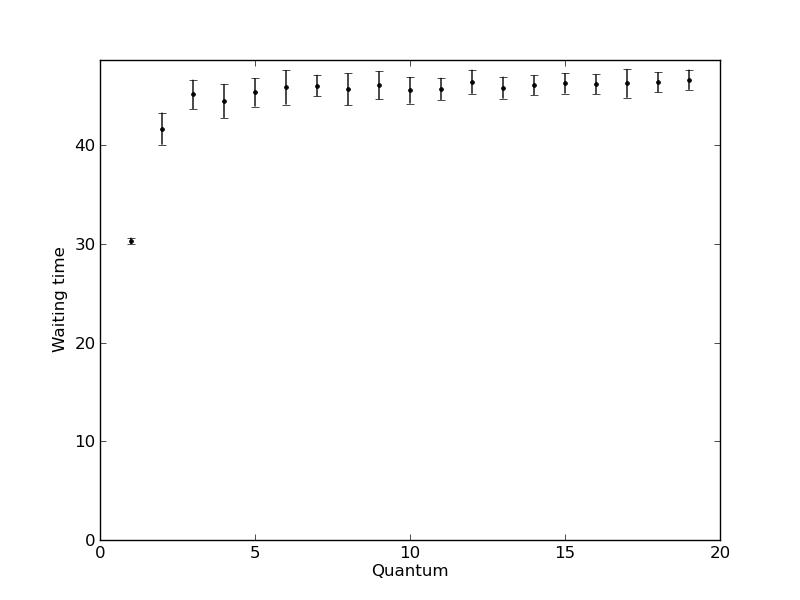
\includegraphics[width=8.75cm]{graficos/cores_2_wt.jpg}}
\hfill
\subfigure[]{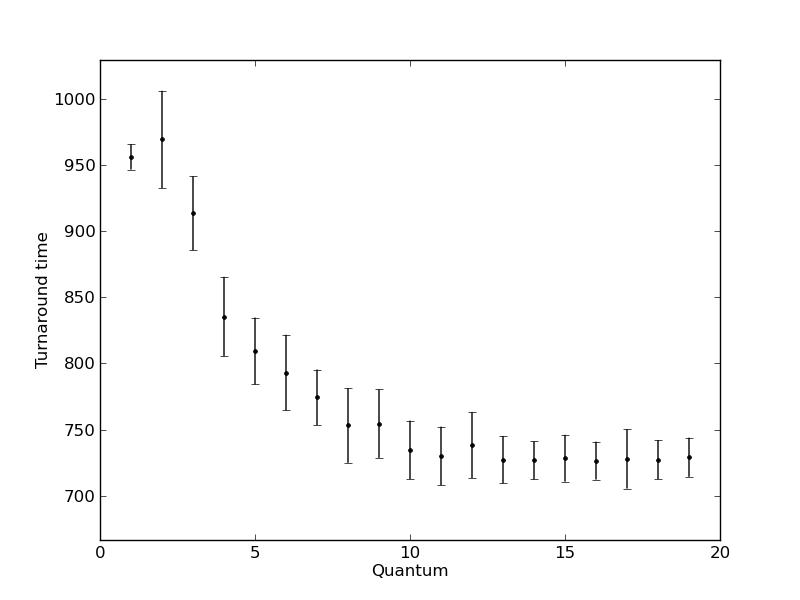
\includegraphics[width=8.75cm]{graficos/cores_2_ta.jpg}}
\hfill
\caption{Representación de Waiting time y Turnaround time en función del quantum para un procesador de 2 núcleos utilizando un lote de tareas $taskBatch$}
\end{figure}

\begin{figure}[H]
\hfill
\subfigure[]{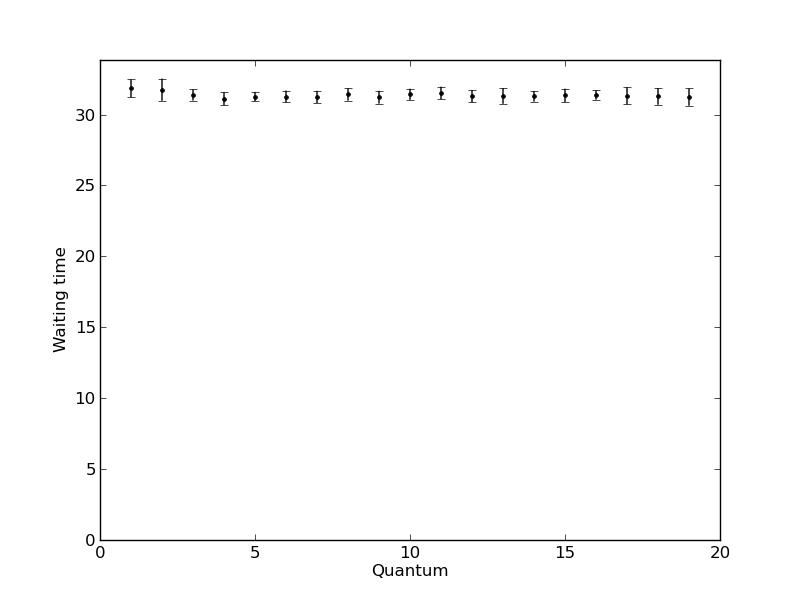
\includegraphics[width=8.75cm]{graficos/cores_3_wt.jpg}}
\hfill
\subfigure[]{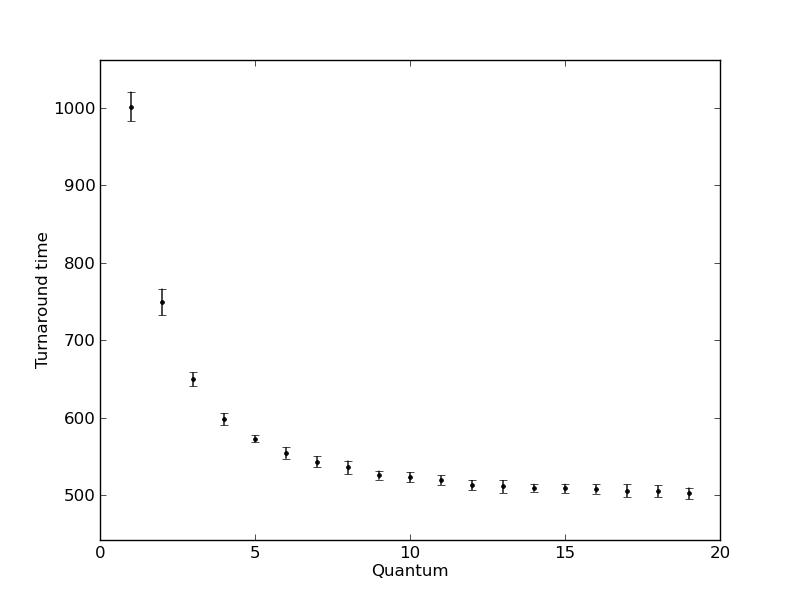
\includegraphics[width=8.75cm]{graficos/cores_3_ta.jpg}}
\hfill
\caption{Representación de Waiting time y Turnaround time en función del quantum para un procesador de 3 núcleos utilizando un lote de tareas $taskBatch$}
\end{figure}

\begin{figure}[H]
\hfill
\subfigure[]{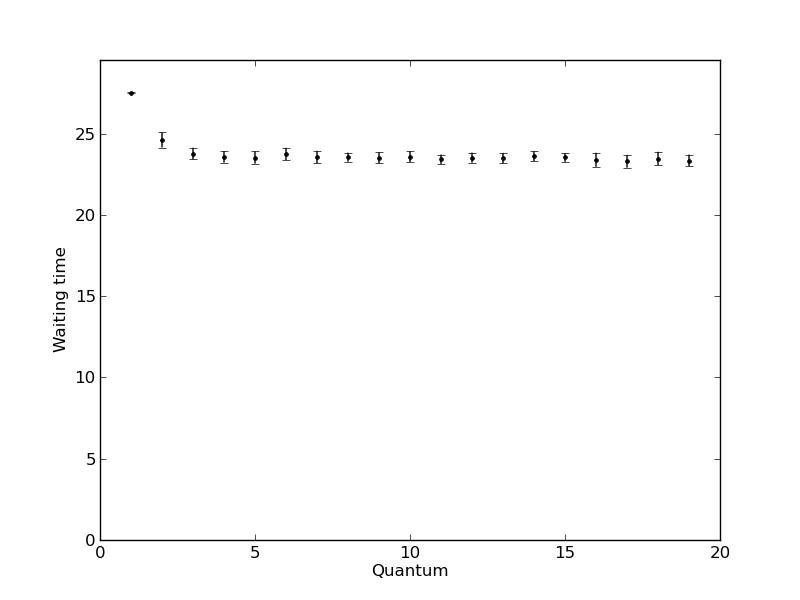
\includegraphics[width=8.75cm]{graficos/cores_4_wt.jpg}}
\hfill
\subfigure[]{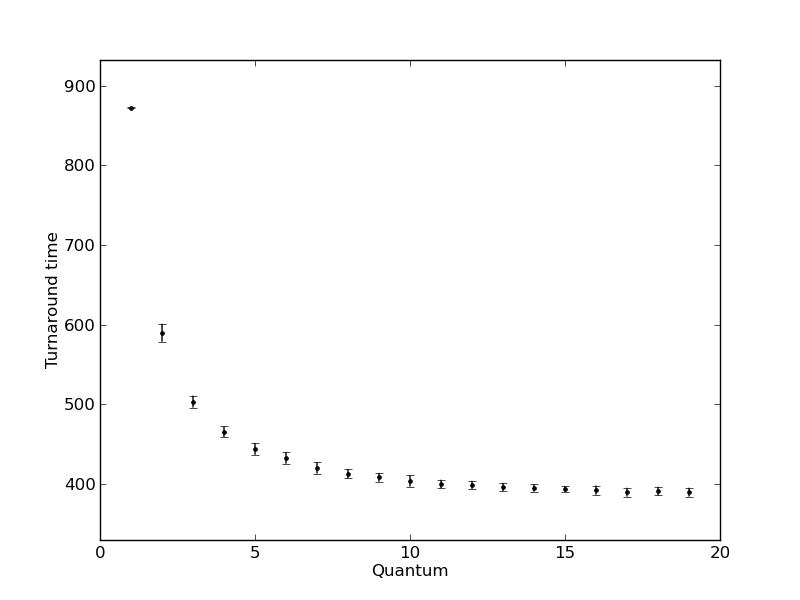
\includegraphics[width=8.75cm]{graficos/cores_4_ta.jpg}}
\hfill
\caption{Representación de Waiting time y Turnaround time en función del quantum para un procesador de 4 núcleos utilizando un lote de tareas $taskBatch$}
\end{figure}

Como puede observarse en las figuras 8, 10 y 12, los valores de waiting time obtenidos no difieren demasiado al ir variando los quantums para cada tarea. Este comportamiento no ocurre en los gráficos de turnaround time en donde comienzan a tenerse resultados similares a partir de un quantum igual a 8. Es por esta razón que nos pareció apropiado determinar un quantum óptimo de 8 ticks para el lote de tareas $TaskBatch$ presentado.

